\documentclass[a4paper]{article}

\usepackage[brazil]{babel}
\usepackage[utf8]{inputenc}
\usepackage{amsmath,amsfonts,amssymb,latexsym,mathrsfs,amsthm,amstext,bezier,amscd}
\usepackage{graphicx}
\usepackage{indentfirst}
\usepackage{setspace}

\begin{document}
\thispagestyle{empty}

\begin{titlepage}
	\vfill
	\begin{center}
		\parbox{6cm}{
\includegraphics[scale=0.2]{logo.png}}\\
		\begingroup
		\fontsize{12pt}{0pt}\selectfont
		{\large \textbf{INSTITUTO FEDERAL DE EDUCAÇÃO, CIÊNCIA E TECNOLOGIA DO CEARÁ}}\\[0.2cm]
		\fontsize{12pt}{0pt}\selectfont
		{\large \textbf{IFCE CAMPUS MARACANAÚ}}\\[0.2cm]
		\fontsize{12pt}{0pt}\selectfont	
		{\large \textbf{BACHARELADO EM CIÊNCIA DA COMPUTAÇÃO}}\\[4cm]
		\fontsize{12pt}{0pt}\selectfont
		{\large \textbf{THIAGO MAGALHÃES FURTADO}}\\[3.5cm]
		\fontsize{12pt}{0pt}\selectfont
		{\large \textbf{Avaliação de Acessibilidade em Portais de Notícias}}\\[3.5cm]
		\fontsize{12pt}{0pt}\selectfont
		{\large \textbf{MARACANAÚ}}\\[0.2cm]
		\fontsize{12pt}{0pt}\selectfont
		{\large \textbf{2021}}
		\endgroup
	\end{center}
\end{titlepage}

\begin{titlepage}
	\vfill
	\begin{center}
		\fontsize{12pt}{0pt}\selectfont
		{\large \textbf{THIAGO MAGALHÃES FURTADO}} \\[2.5cm]
		\fontsize{12pt}{0pt}\selectfont
		{\large \textbf{Avaliação de Acessibilidade em Portais de Notícias}}\\[3cm]
		
		\hspace{.45\textwidth} %posiciona a minipage
		\begin{minipage}{.5\textwidth}
			\large Trabalho de Conclusão de Curso apresentado ao curso de Bacharelado em Ciência da Computação do Instituto Federal de Educação, Ciência e Tecnologia do Ceará (IFCE) - Campus Maracanaú, como requisito parcial para obtenção do Título de Bacharel em Ciência da Computação.\\[1cm]
			Prof. Dr. Otávio Alcântara de Lima Junior.
		\end{minipage}
		\vfill
		\vspace{2cm}		
		\large \textbf{Maracanaú - CE}
		
		\large \textbf{2021}
	\end{center}
\end{titlepage}

\begin{titlepage}
	\begin{center}
		\tableofcontents
	\end{center}
\end{titlepage}
\begin{titlepage}
\section{INTRODUÇÃO}
\fontsize{12pt}{0pt}\selectfont
\onehalfspacing
Estamos vivendo em uma época em que a tecnologia tem avançado bastante, isso é notório se nós analisarmos as três últimas décadas, durante as quais o mundo entrou na chamada era da informação. Assim, os computadores, a Internet, os acessos aos sites e o número de usuários, em todo o mundo, têm tido avanços significativos. Esses avanços possibilitam, para a nossa sociedade, uma prestação de serviço e uma obtenção de informação rápida. Porém, muitos sites não possibilitam uma navegação agradável e tranquila à todos, já que alguns usuários tem dificuldade para acessá-los, por possuírem alguma deficiência, a OMS relata que 15\% da população mundial tem alguma deficiência [1].

Dentre a diversidade de conteúdo da Internet, pode-se destacar os portais de noticiais como ferramentas importantes para divulgação de informação de qualidade para a sociedade. Porém essas plataformas digitais precisam alcançar todos os usuários, inclusive os PCDs(pessoas com deficiência). Para avaliar a acessibilidade desses sites, é necessário a aplicação de diretrizes de acessibilidade que são propostas por instituições e governos. Por exemplo, a eMAG é uma diretriz proposta pelo governo brasileiro em 2004, utilizada por algumas plataformas digitais nacionais [2].

Outra diretriz usada atualmente é a WCAG (Web Content Accessibility Guidelines), que já está na sua segunda versão, isto é, a WCAG 2.0. A WCAG possuí doze diretrizes organizadas em quatro princípios diferentes, possuindo algumas recomendações para cada princípio [3], que são indispensáveis em qualquer plataforma digital, inclusive nos sites de notícia.

O WCAG é um padrão adotado em diversos trabalhos de avaliação de acessibilidade, em [4], foi avaliado a acessibilidade dos vídeos na plataforma online de curso MOOC. Foram analisados os vídeos através da verificação do uso de uma alternativa à informação visual, de audiodescrição, transcrições, de uma fonte boa, com um tamanho de letra razoável e de alto-contraste. Em o [5] e em [6] foi analisado a existência de acessibilidade dos sites de ensino do nível superior da Índia utilizando o WCAG e uma ferramenta de avaliação, chamada de TAW. Em 2016, foi feito um acompanhamento, por meio do WCAG, dos serviços de governo eletrônico da Arábia Saudita, com o objetivo de analisar o nível de conscientização e as políticas do próprio governo [7]. Por fim, em [8], foi feito uma analise de um método heurístico existente para investigar o nível de acessibilidade de 40 sites em relação aos usuários com baixa visão juntamente com a diretriz WCAG 2.1, o método utilizado foi proposto por Brajnik.

Este artigo propõe a avaliação de acessibilidade de dez dos principais portais de notícias brasileiros, que tem um papel importantíssimo em relação ao repasse de informação para o público em geral, inclusive para os usuários PCDs, supondo que eles não atendem de forma plena os requisitos desse público. Para isso será proposto uma avaliação da acessibilidade de dez sites de notícia para pessoas que possuem algum grau de deficiência visual ou auditiva. A pesquisa tem o intuito de analisar os sites, de forma plena, para quantificar o grau de acessibilidade de cada um. Assim, o objetivo geral do trabalho é avaliar sites de notícias que possuem formas de acessibilidade digital, sejam completamente, parcialmente ou não acessíveis para a deficiência visual e para a deficiência auditiva. A metodologia empregada consiste em caracterizar a definição de acessibilidade digital, verificar as formas de deficiência existentes que afetam a usabilidade dos sites, apresentando a diretriz WCAG, escolhendo os princípios destinados aos deficientes visuais e auditivos para mensurar os sites de notícias em relação a acessibilidade.

O restante do artigo está organizado da seguinte forma. Na seção 2 será mostrado a metodologia que será aplicada para fazer a analise dos sites. Na seção 3 será apresentado o estado da arte de avaliação de acessibilidade em sites usando as diretrizes, mostrando quais diretrizes usaram e em quais plataformas aconteceram as suas pesquisas. Na seção 4 serão explicadas as formas de deficiência existentes que afetam a usabilidade dos sites. Na seção 5 será analisado a diretriz WCAG. Na seção 6 será apresentado os pontos fortes e fracos dos sites de notícias relacionado com a acessibilidade web através da análise da diretriz com o propósito de fazer sugestões de melhorias. Por fim, na seção 7 será apresentada uma discussão sobre os resultados da avaliação de acessibilidade e a conclusão do trabalho.

\section{METODOLOGIA}
Essa pesquisa escolheu os sites de notícia pelo fato deles terem um papel bastante importante para a sociedade atual, já que eles tem o compromisso de informar para cada pessoa, que as acessa, o que está acontecendo no Brasil e no mundo.

Sendo assim, será primeiro explicado as formas de deficiências existentes que afetam a visão e audição. Após isso será apresentado a diretriz WCAG mostrando cada um dos seus princípios. Assim, apontando cada um dos seus princípios, será feito uma analise dos dez sites notícia para averiguar a acessibilidade de cada um deles. Tudo isso para computar o grau de acessibilidade de cada um desses sites. Então, a metodologia, que será aplicada para que os objetivos sejam alcançados, será:

1 - Mostrar e explicar as formas de deficiência visual e auditiva;

2 - Analisar a WCAG;

3 - Pontuar os princípios e as especificações da diretriz WCAG;

4 - Apontar as principais formas de acessibilidade, usando a diretriz WCAG;

5 - Escolher dez sites de notícias do Brasil;

6 - Fazer um levantamento da acessibilidade de cada site de acordo com as especificações;

7 - Fazer uma pesquisa para saber como computar os sites;

8 - Fazer um comparativo do resultado da computação entre os sites;

9 - Apresentar a conclusão tirada dos dez sites escolhidos, propondo melhorias em cada um deles.

Todos os passos da metodologia que será aplicada estão descritos na Figura 1.\\

Figura 1 - Fluxograma das etapas da metodologia\\[-0.7cm]
\begin{center}
	\parbox{10cm}{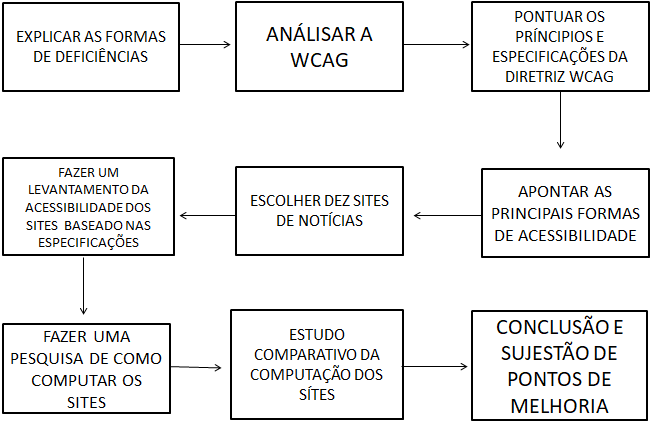
\includegraphics[scale=0.6]{Fluxograma - Metodologia TCC.png}}
\end{center}

Portanto, esse será o caminho percorrido por esse artigo. A seguir, será mostrado todo o cronograma para se cumprir cada ponto listado acima.

\section{CRONOGRAMA}
Sobre o cronograma do artigo, foram propostos os seguintes passos, baseado na metodologia, com suas respectivas datas como visto na tabela abaixo.

Tabela 1 - Cronograma da pesquisa\\
\begin{center}
	\fontsize{8pt}{8pt}\selectfont
	\begin{tabular}{|cccccccc|}
		\hline
		Atividades & 05 à & 08/21 & 09/21 & 10/21 & 11 à & 01 à & 03 à\\
		 & 07/21 & & & & 12/21 & 02/22 & 04/22\\
		\hline
		Bibliografia & X & & & & & & \\
		e apresentação & & & & & & & \\
		da WCAG & & & & & & & \\
		\hline
		Explicar as formas & & X & & & & & \\
		de deficiência & & & & & & & \\
		\hline
		Mostrar princípios e & & & X & & & & \\
		especificações da WCAG & & & & & & & \\
		\hline
		Apontar as & & & & X & & & \\
		principais formas & & & & & & & \\
		de acessibilidade & & & & & & & \\
		\hline
		Analisar os & & & & & X & & \\
		sites conforme & & & & & & & \\
		a WCAG & & & & & & & \\
		\hline
		Computar a & & & & & & X & \\
		acessibilidade & & & & & & & \\
		de cada site & & & & & & & \\
		\hline
		Divulgação dos & & & & & & & X \\
		resultados e & & & & & & & \\
		conclusão & & & & & & & \\
		do artigo & & & & & & & \\
		\hline
	\end{tabular}
\end{center}

Assim, esse será o cronograma estimado para esse artigo. A seguir, será apresentado os trabalhos relacionados sobre acessibilidade digital e sobre as diretrizes.

\section{TRABALHOS RELACIONADOS}
Há uma grande produção nessa área, contudo serão concentrados os artigos publicados em revistas. Será mostrado os artigos que tratam sobre as diretrizes utilizadas nos respectivos estudos e sobre as propostas de avaliação em diversas áreas, sejam elas em portais de notícia ou não.

\subsection{Diretrizes}
Sobre as diretrizes, serão apresentados alguns trabalhos que focaram em duas diretrizes, que são a eMAG e a WCAG. 

A WCAG, publicada pela World Wide Web (W3C) no dia primeiro de outubro de 1994, através da organização chamada World Wide Consortium, que é um consórcio com 450 membros, empresas, organizações independentes e ONGs, tem como objetivo formular padrões para os desenvolvedores criarem seus sites. Segundo o artigo [3] a WCAG 2.0, tem como objetivo eliminar erros de acessibilidade através dos web designers e dos desenvolvedores. Assim, ela serve de apoio para os desenvolvedores a boa prática da acessibilidade web, garantindo um acesso à internet satisfatório, atingindo o maior número de pessoas possível, independente da existência de uma comorbidade física.

Segundo a documentação da WCAG [10], onde a ultima versão foi publicada em 11 de dezembro de 2008, é mostrada as recomendações, explicando, sucintamente, os seus quatro princípios. O primeiro princípio é o perceptível, no qual informação e os componentes da interface de utilizador têm que ser apresentados de forma a que os utilizadores as possam entender. Nesse princípio existem quatro diretrizes com suas especificações. As diretrizes determinam que os sites precisam ter alternativas em texto, ter uma mídia dinâmica e contínua, ser adaptável e ser distinguível.

O site ter alternativas em texto significa que ele deve fornecer alternativas em texto para todo o conteúdo não textual de modo que possa ser apresentado de outras formas, de acordo com as necessidades dos utilizadores. Alguns exemplos são caracteres ampliados, braille, fala, símbolos ou uma linguagem mais simples. Ja o site ter um mídia dinâmica ou contínua remete que ele deve fornecer alternativas para conteúdo em multimédia dinâmica ou temporal. A diretriz adaptável diz que deve ser criado um conteúdo que possa ser apresentado de diferentes formas, por exemplo, um esquema de página mais simples, sem perder informação ou estrutura. Por fim, a diretriz distinguível expressa que deve haver uma facilitação dos utilizadores à audição e à visão dos conteúdos nomeadamente através da separação do primeiro plano do plano de fundo. Todas as diretrizes do princípio perceptível estão especificadas e descritas, logo abaixo, na figura 2.\\

Tabela 2 - Diretrizes do princípio perceptível\\
\begin{center}
	\fontsize{8pt}{8pt}\selectfont
	\begin{tabular}{|cc|}
		\hline
		Diretrizes & Especificações \\
		\hline
		Diretriz 1.1 Alternativas& 1.1.1 Conteúdo Não Textual\\
		em Texto & \\
		\hline
		Diretriz 1.2 Mídia & 1.2.1 Conteúdo só de áudio\\
		Dinâmica ou Contínua & e só de vídeo (pré-gravado) \\
		& 1.2.2 Legendas (pré-gravadas)\\
		& 1.2.3 Audiodescrição ou Alternativa\\
		& em Multimídia (pré-gravada)\\
		& 1.2.4 Legendas (em direto)\\
		& 1.2.5 Audiodescrição (pré-gravada)\\
		& 1.2.6 Língua Gestual (pré-gravada)\\
		& 1.2.7 Audiodescrição Alargada (pré-gravada)\\
		& 1.2.8 Alternativa em Multimídia (pré-gravada)\\
		& 1.2.9 Só áudio (em direto)\\
		\hline
		Diretriz 1.3 Adaptável& 1.3.1 Informações e Relações\\
		& 1.3.2 Sequência com Significado\\
		& 1.3.3 Características Sensoriais\\
		\hline
		Diretriz 1.4 Distinguível& 1.4.1 Utilização da Cor\\
		& 1.4.2 Controle de Áudio\\
		& 1.4.3 Contraste\\
		& 1.4.4 Redimensionar texto\\
		& 1.4.5 Imagens de Texto\\
		& 1.4.6 Contraste (Melhorado)\\
		& 1.4.7 Som Baixo ou Ausência de Som de Fundo\\
		& 1.4.7 Ausência de Fundo, Desligar\\
		& 1.4.8 Apresentação Visual\\
		& 1.4.9 Imagens de Texto (sem exceção)\\
		\hline
	\end{tabular}
\end{center}

Já o segundo princípio é o operável, onde é definido os métodos, que possibilitam, para os usuários, uma interação e uma boa navegação pelo conteúdo de forma confortável. O princípio diz que os sites devem usar interfaces apropriadas para os deficientes, isto é, os componentes da interface de utilizador e a navegação têm de ser operáveis. Nesse princípio existem quatro diretrizes com suas especificações. As diretrizes determinam que o site deve ser acessível por teclado, deve ter um tempo suficiente, não deve causar convulsões e ele deve ser navegável.

Dizer que a plataforma digital deve ser acessível por teclado exprime que ela deve ter uma funcionalidade que fique disponível a partir do teclado. Já o site ter um tempo suficiente revela que ele deve proporcionar aos utilizadores um tempo suficiente para lerem e utilizarem o conteúdo. Sobre o site não causar convulsões, pressupõe-se que ele não deve criar conteúdos de uma forma que se sabe que pode causar convulsões em alguns usuários. E, por último, dizer que a página da Internet deve ser navegável, representa que ela deve fornecer formas de ajudar os utilizadores a navegar, localizar conteúdos e determinar o local onde estão. Todas as diretrizes do princípio operável estão especificadas e descritas, logo abaixo, na figura 3.\\

Tabela 3 - Diretrizes do princípio operável\\
\begin{center}
	\fontsize{8pt}{8pt}\selectfont
	\begin{tabular}{|cc|}
		\hline
		Diretrizes & Especificações \\
		\hline
		Diretriz 2.1 Acessível por Teclado& 2.1.1 Teclado\\
		& 2.1.2 Sem bloqueio do teclado\\
		& 2.1.3 Teclado(Sem Exceção)\\
		\hline
		Diretriz 2.2 Tempo Suficiente & 2.2.1 Tempo ajustável \\
		& 2.2.2 Colocar em pausa, parar, ocultar\\
		& 2.2.3 Sem temporização\\
		& 2.2.4 Interrupções\\
		& 2.2.5 Nova autenticação\\
		\hline
		Diretriz 2.3 Convulsões& 2.3.1 Três Flashes ou Abaixo do Limite\\
		& 2.3.2 Três Flashes\\
		\hline
		Diretriz 2.4 Navegável& 2.4.1 Ignorar Blocos\\
		& 2.4.2 Página com Título\\
		& 2.4.3 Ordem do Foco\\
		& 2.4.4 Finalidade da\\
		& 2.4.4 Hiperligação (Em Contexto)\\
		& 2.4.5 Várias Formas\\
		& 2.4.6 Cabeçalhos e Etiquetas\\
		& 2.4.7 Foco Visível\\
		& 2.4.8 Localização\\
		& 2.4.9 Finalidade da Hiperligação\\
		& 2.4.9 (Apenas a Hiperligação)\\
		& 2.4.10 Cabeçalhos da Secção\\
		\hline
	\end{tabular}
\end{center}

O terceiro princípio é o compreensível, que diz que os usuários devem ser capazes de compreender as informações e o funcionamento da interface, com o objetivo do usuário interpretar corretamente o conteúdo da plataforma digital, isto é, a informação e a utilização da interface de utilizador têm de ser compreensíveis. Nesse princípio existem três diretrizes com suas especificações. As diretrizes determinam que o site deve ser legível, deve ser previsível e deve existir assistência na Inserção de Dados.

Dizer que o sítio da Internet deve ser legível simboliza que ele é capaz de tornar o conteúdo textual legível e compreensível. Já falar que o sítio eletrônico tem que ser previsível reflete a ideia de fazer com que as páginas Web apareçam e funcionem de forma previsível. E existir na página Web uma assistência na inserção de dados, retrata que ela deve ajudar os utilizadores a evitar e a corrigir os erros. Todas as diretrizes do princípio compreensível estão especificadas e descritas, logo abaixo, na figura 4.\\

Tabela 4 - Diretrizes do princípio compreensível\\
\begin{center}
	\fontsize{8pt}{8pt}\selectfont
	\begin{tabular}{|cc|}
		\hline
		Diretrizes & Especificações \\
		\hline
		Diretriz 3.1 Legível& 3.1.1 Idioma da página\\
		& 3.1.2 Idioma das partes\\
		& 3.1.3 Palavras invulgares\\
		\hline
		Diretriz 3.2 Previsível & 3.2.1 Ao receber o Foco\\
		& 3.2.2 Ao entrar num campo\\
		& de edição (input)\\
		& 3.2.3 Consistência de Navegação\\
		& 3.2.4 Consistência de Identificação\\
		& 3.2.5 Alteração a Pedido\\
		\hline
		Diretriz 3.3 Assistência na Inserção de Dados& 3.3.1 Identificação de Erros\\
		& 3.3.2 Etiquetas ou Instruções\\
		& 3.3.3 Sugestão para eliminar o Erro\\
		& 3.3.4 Prevenção de Erros\\
		& (Legais, Financeiros, Dados)\\
		& 3.3.5 Ajuda\\
		& 3.3.6 Prevenção de Erros\\
		& (de qualquer tipo)\\
		\hline
	\end{tabular}
\end{center}
Por fim, o quarto e último princípio é o robusto, que foca na grande variedade dos usuários poderem interpretar o conteúdo da maneira mais confiável possível, além de levar, em consideração, a compatibilidade com as tecnologias atuais e futuras. Isso tem a finalidade de maximizar a harmonização das páginas da web com os seus usuários e com essas tais tecnologias, isto é, o conteúdo deve ser suficientemente robusto para ser interpretado de forma fiável por uma ampla variedade de agentes utilizadores da plataforma em questão, incluindo as tecnologias de apoio. Nesse princípio existe apenas uma diretriz com suas especificações, A diretriz determina que o site deve ser compatível, isto é, ele deve maximizar a compatibilidade com os agentes de utilizador atuais e futuros, incluindo as tecnologias de apoio. Essa única diretriz do princípio compreensível está especificada e descrita, logo abaixo, na figura 5.\\

Tabela 5 - Diretrizes do princípio robusto\\[-0.7cm]
\begin{center}
	\fontsize{8pt}{8pt}\selectfont
	\begin{tabular}{|cc|}
		\hline
		Diretrizes & Especificações \\
		\hline
		Diretriz 4.1 Compatível& 4.1.1 Análise sintática (parsing)\\
		& 4.1.2 Nome, Função, Valor\\
		\hline
	\end{tabular}
\end{center}

Mas na frente na seção 5, serão detalhadas as especificações, porém, com o que já foi apresentado, é visto que as diretrizes são bem extensa e abrange quase todas as formas de acessibilidade existentes. Agora é preciso só que os programadores se propõem a seguir os quatro princípios básicos ditos anteriormente, com a meta de fazer tal atividade em seus trechos de códigos, fazendo com que todas as pessoas consigam manipular os seus sites, sem haver nenhum tipo de discriminação por partes dos programadores e dos produtores de conteúdos.

\subsection{Avaliação de Acessibilidade de Sites}
Nesta subseção são apresentados artigos sobre avaliação de acessibilidade de sites de diferentes campos.  No artigo [1] os autores avaliaram 107 sites educacionais no Brasil, através da existência dos seguintes pontos, atalhos de teclado, alto contraste, barra de acessibilidade, mapa de sitio e paginas com descrições, chegando a conclusão que há um elevado descaso com a inclusão digital em relação às pessoas com deficiência. Já em [7], foi feito uma analise da acessibilidade dos sites governamentais da Arábia Saudita, analisando a existência de uma boa informação de conteúdo não textual e seus relacionamentos, de contraste, de imagens de texto e vídeos de libras, de atalhos de teclado, de interrupções e de uma boa sequência significativa. Segundo eles, os resultados da avaliação são promissores e indicam um aumento da conscientização para acessibilidade da web.

Já o artigo [9] tinha como objetivo investigar os sites de governo eletrônico móvel. Chegaram a conclusão que há problemas de usabilidade e acessibilidade que afetam o desempenho de sites governamentais. Dentre os pontos analisados, estão a existência de texto alternativo as imagens, alto contraste no texto, descrição dos link, formulários de fácil compreensão e textos, em gerais, que favoreçam o uso dos leitores de tela, que são usados caso tenham uma boa sequência significativa. O artigo [11] tinha como objetivo deste avaliar a acessibilidade de 91421 vídeos de 113 universidades do mundo. Os resultados deste estudo mostram que embora apenas 17\% do total de vídeos publicados tenham legendas associadas, mas o cumprimento deste critério de sucesso tem melhorado ao longo dos anos. Porém, não existe acessibilidade em relação à linguagem de sinais, à descrição de áudio ou à descrição de áudio estendida com vídeos, a acessibilidade é zero.

A seguir, na tabela 1, vemos a comparação dos artigos citados nessa seção com as características da diretriz WCAG.\\

Tabela 1 - Análise características das diretrizes com os artigos.
\begin{center}
	\begin{tabular}{cc}
		\hline
		Artigos & Diretrizes cumpridas\\
		\hline
		Artigo [1] & 1.2.3/1.2.5/1.2.7/1.4.3/1.4.5/1.4.6/1.4.9/2.1.1/2.1.2/2.1.3\\
		Artigo [7] & 1.2.6/1.3.2/1.4.3/1.4.5/1.4.6/1.4.9/2.1.1/2.1.2/2.1.3/2.2.4\\
		Artigo [9] & 1.2.8/1.2.9/1.3.2/1.4.3/1.4.5/1.4.6/1.4.9/4.1.2\\
		Artigo [11] & 1.1.1/1.2.1/1.2.2/1.2.3/1.2.4/1.2.5/1.2.6\\
		\hline
	\end{tabular}
\end{center}

Já o artigo [8] foi analisado um método heurístico existente para investigar o nível de acessibilidade de 40 sites, incluindo os de 30 universidades da América Latina e 10 sites entre os mais visitados. Foram analisados em relação aos usuários com baixa visão, o método utilizado foi proposto por Brajnik e WCAG 2.1 chamado de Testes de Triagem de Barreiras. Esta técnica consiste em priorizar os impactos das barreiras de acordo com o contexto aplicado. O método permite a identificação da gravidade de cada barreira buscando identificar problemas de acessibilidade. Assim, o artigo concluiu, que muitas nas páginas web analisadas foi violado alguns princípios da diretriz WCAG, totalizando 241 barreiras.

\section{TIPOS DE DEFICIÊNCIA}
Nesta seção será detalhado, de forma sucinta, as mais variadas formas de deficiência visual e auditiva.

\subsection{Formas de deficiência visual}
Sobre a deficiência visual se divide em dois grupos com características e necessidades diferentes. Os dois grupos de pessoas são aqueles que apresentam baixa visão e aqueles com cegueira.

Cegueira é usado para identificar a condição de pessoas que apresentam total incapacidade de enxergar e também para aquelas com uma visão residual que, apesar de não ser a perda total da visão, dificulta-as de realizar suas atividades diárias normalmente.

Assim, o cego é aquele que não utiliza a visão para a aprendizagem e que necessita de sistemas Braille ou de sistemas que verbalizam textos em computadores. Baixa visão ou visão subnormal é o termo usado para a pessoa que tem sua função visual comprometida, mas que usa ou é potencialmente capaz de usar a visão para executar tarefas.

Já a pessoa que possui baixa visão tem uma condição na qual a sua não pode ser totalmente corrigida por óculos, interferindo em suas atividades diárias, assim como a leitura e a locomoção. A baixa visão é pode ser causado pela degeneração macular, glaucoma, retinopatia diabética, ou catarata. As pessoas com baixa visão necessitam do uso de óculos, lentes corretivas, lupas simples e/ou eletrônicas, além de caracteres ampliados e de uso de tecnologias assistivas como alto contraste e leitores de tela.

Portanto, os usuários que possuem alguma deficiência visual são altamente prejudicados quando precisam acessar uma plataforma digital, pois eles ficam impossibilitados de usá-la pelo o fato delas não terem determinadas funcionalidades. Por exemplo, a falta de alto contraste afeta pessoas que possuem o daltonismo, elas necessitam de sites que são completamente pretos e brancos. Além disso, as pessoas que não conseguem ler determinadas palavras pelo tamanho da letra, isto é, pessoas que possuem baixa visão, elas precisam da funcionalidade de aumentar a fonte, com o objetivo de enxergarem tudo que o site propõe mostrar aos seus usuários, por fim existem aquelas pessoas que possuem a cegueira total, isto é, são aqueles que tem a total incapacidade para ver o mundo exterior. Portanto, esses são os exemplos das deficiências visuais que afetam a usabilidade dos usuários ao estarem acessando as plataformas digitais, a seguir iremos falar sobre a diversidade da deficiência auditiva.

\subsection{Formas de deficiência auditiva}
Sobre a deficiência auditiva é considerada como a diferença existente entre o desempenho do indivíduo e a habilidade normal para a detecção sonora. Considera-se, em geral, que a audição normal corresponde à habilidade para detecção de sons até 20 dB N.A (decibéis, nível de audição). A audição serve para o desenvolvimento e na manutenção da comunicação por meio da linguagem falada.

Dentre os exemplos de deficiência auditiva está a condutiva, que ocorre quando qualquer interferência na transmissão do som desde o conduto auditivo externo até a orelha interna. A grande maioria das deficiências auditivas condutivas pode ser corrigida através de tratamento clínico ou cirúrgico. Esta deficiência pode ter várias causa, entre elas pode-se citar, os corpos estranhos no conduto auditivo externo, tampões de cera , otite externa e média, mal formação congênita do conduto auditivo, inflamação da membrana timpânica, perfuração do tímpano, obstrução da tuba auditiva, etc.

Já a sensório-neural é quando há uma impossibilidade de recepção do som por lesão das células ciliadas da orelha interna ou do nervo auditivo. Este tipo de deficiência auditiva é irreversível. A deficiência auditiva sensório-neural pode ser de origem hereditária como problemas da mãe no pré-natal tais como a rubéola, sífilis, herpes, toxoplasmose, alcoolismo, toxemia, diabetes etc. Também podem ser causadas por traumas físicos, prematuridade, baixo peso ao nascimento, trauma de parto, meningite, encefalite, caxumba, sarampo etc.

A mista é quando há uma alteração na condução do som até o órgão terminal sensorial associada à lesão do órgão sensorial ou do nervo auditivo. O audiograma mostra geralmente limiares de condução óssea abaixo dos níveis normais, embora com comprometimento menos intenso do que nos limiares de condução aérea.

Por fim, a central ou surdez central não é, necessariamente, acompanhado de diminuição da sensitividade auditiva, mas manifesta-se por diferentes graus de dificuldade na compreensão das informações sonoras. Decorre de alterações nos mecanismos de processamento da informação sonora no tronco cerebral.

Os níveis de limiares utilizados para caracterizar os graus de severidade da deficiência auditiva são, audição normal, limiares entre 0 a 24 dB nível de audição. Deficiência auditiva leve, limiares entre 25 a 40 dB nível de audição. Deficiência auditiva moderna, limiares entre 41 e 70 dB nível de audição. Deficiência auditiva severa, limiares entre 71 e 90 dB nível de audição. Deficiência auditiva profunda, limiares acima de 90 dB.

Entre os muitos instrumentos usados para comunicação não oral, figura a linguagem dos sinais, criada por um monge beneditino francês, morador de um mosteiro onde imperava a lei do silêncio. Adotada há mais de cem anos, no Brasil é chamada de Libras. Assim esses são os exemplos das deficiências auditivas que afetam o acesso de forma tranquila dos sites, inclusive os jornalísticos, a seguir iremos analisar a diretriz WCAG.

\section{ANÁLISE DA DIRETRIZ WCAG}

\section{ANÁLISE DOS SITES DE NOTÍCIA}

\section{CONCLUSÃO}

\section*{REFERÊNCIAS}
\addcontentsline{toc}{section}{Referência}
\hspace{-0.05\textwidth}
\begin{minipage}{1\textwidth}
[1] M. Campoverde-Molina, S. Lujan-Mora, e L. Valverde Gracia, "Empirical Studies on Web Accessibility of Educational Websites: A Systematic Literature Review" em IEEEAcess, Abril de 2020.
\end{minipage}\\[0.5cm]
[2] D. Luís Arenhardt, T. Stefanel Franchi, e S. Medianeira Flores Costa, M. Zampieri Grohmann, "Acessibilidade digital: Uma análise em portais de Instituições Federais de Educação do Brasil" em Education Policy Analysis Archives, Abril de 2017.\\[0.5cm] [3] P. Acosta-Vargas, T. Acosta, e S. Luján-Mora, "Challenges to Assess Accessibility in Higher A Comparative Study of Latin America Universities" em IEEEAcess, Março de 2018.\\[0.5cm] [4] E. M. Molanes-López, A. Rodriguez-Ascaso, E. Letón, E J. Pérez-Martín, "Assessment of Video Accessibility by Students of a MOOC on Digital Materials for All a MOOC on Digital Materials for All" em IEEEAcess, Maio de 2021.\\[0.5cm] [5] A. Ismail, K. S. Kuppusamy, "Web accessibility investigation and identification of major issues of higher education websites with statistical measures - A case study of college websites" em Journal of King Saud University – Computer and Information Sciences, Março de 2019.\\[0.5cm] [6] A. Ismail, K. S. Kuppusamy, "Accessibility of Indian universities homepages An exploratory study" em Journal of King Saud University – Computer and Information Sciences, Junho de 2016.\\[0.5cm] [7] H. S. Al-Khalifa, I. Baazeem e R. Alamer1, "Revisiting the accessibility of Saudi Arabia government websites" em Universal Access in the Information Society, Setembro de 2016.\\[0.5cm] [8] P. Acosta-Vargas, T. Acosta, e S. Luján-Mora, "A Heuristic Method to Evaluate Web Accessibility for Users With Low Vision" em IEEEAcess, Março de 2018.\\[0.5cm] [9] H. O. Al-Sakran, M. A, Alsudairi "Usability and Accessibility Assessment of Saudi Arabia Mobile E-Government Websites" em IEEEAcess, Março de 2021.\\[0.5cm] [10] B. Caldwell, M. Cooper, L. Guarino Reid, G. Vanderheiden, W. Chisholm, J. Slatin e J. White, Consórcio W3C(2008), "Diretrizes de Acessibilidade para Conteúdo Web (WCAG)2.0", Acesso em: 11 jun. 2021. [Online]. Disponível: https://www.w3.org/Translations/WCAG20-pt-PT/WCAG20-pt-PT-20141024/\\[0.5cm] [11] T. Acosta, P. Acosta Vargas, J. Zambrano Miranda e S. Luján Mora, "Web Accessibility Evaluation of Videos Published on YouTube by Worldwide Top-Ranking Universities" em IEEEAcess, Junho de 2020.

\end{titlepage}
\end{document}